\documentclass{cv}

\usepackage[francais]{babel} 
\usepackage[utf8]{inputenc}  %% les accents dans le fichier.tex
\usepackage[T1]{fontenc}       %% Pour la césure des mots accentués
\usepackage[paper=a4paper,textwidth=160mm]{geometry}
\usepackage{graphicx}
\usepackage{url}                % citer des adresses électroniques et des URL
\usepackage{vmargin}            % redéfinir les marges
\usepackage[usenames, dvipsnames]{color}
\setmarginsrb{1cm}{1cm}{1cm}{1cm}{0cm}{0cm}{0cm}{0cm}


\newcommand{\lieu}[1]{{#1}\ }
\newcommand{\activite}[1]{\textbf{#1}\ }
\newcommand{\comment}[1]{\textsl{#1}\ }
\newcommand{\fonction}[1]{\textbf{#1}\ }

\begin{document}

\begin{center}
\color{OliveGreen}
\par\textbf{\LARGE \textsc{Erwan ROUZEL}}\\
\color{Black}
\color{RoyalBlue}\textbf{\textsc{\large{Ingénieur Logiciel Senior -- Etudiant Ecole Centrale Paris}}}
\color{Black}
\\
\vspace{0.4cm}
\textit{\large{Java -- Architecture -- Cloud -- Big Data -- Mobile -- Méthodes Agiles -- Bilingue}}

\vspace{0.2cm}

\end{center}

\begin{chapeau}

\begin{adresse}
	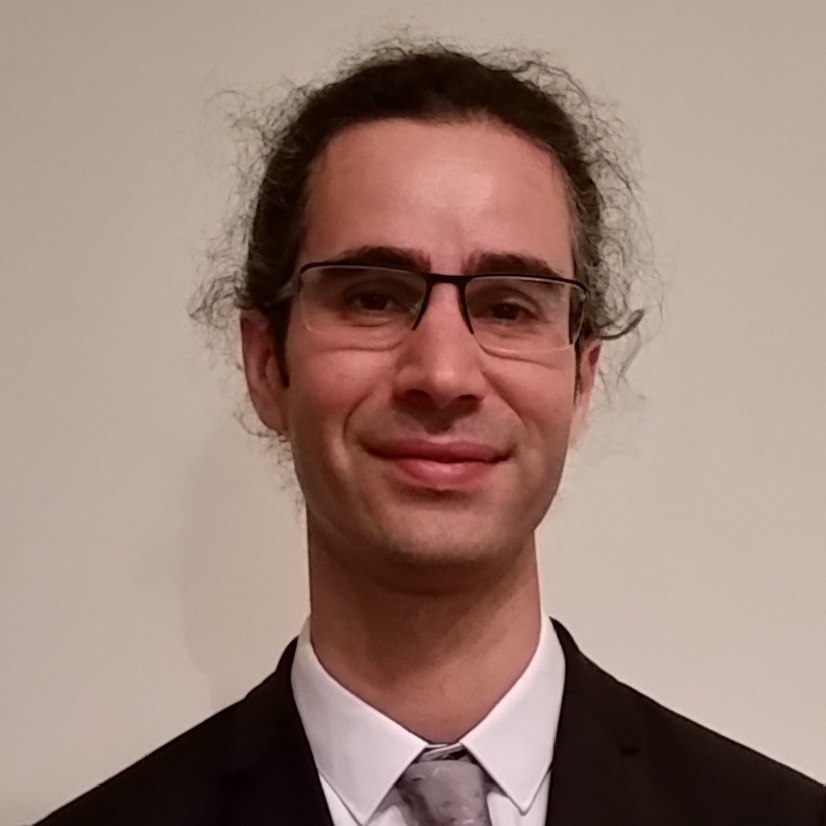
\includegraphics[width=3.75cm,height=3.75cm]{photo-cv-erwan-2016.jpg}
\end{adresse}
\begin{etatcivil}
	Né le 14/09/1981\\
	marié, 1 enfant, permis B
	\linebreak \linebreak
	41, rue hoffmann\\%
	92340 Bourg-la-Reine
	\linebreak

06 85 43 56 33\\
\url{erwan.rouzel@sio.ecp.fr}

\raisebox{-0.55ex}{
\includegraphics[width=2.5ex]{icon-linkedin}}%
\hspace{0.2cm}\url{linkedin.com/in/erouzel}

\end{etatcivil}
\end{chapeau}

\vspace{0.1cm}

\begin{rubriquetableau}[18cm]{OliveGreen}{Projet professionnel}
\textbf{Je suis curieux, ouvert d’esprit et j’aime explorer de nouvelles voies. Après avoir travaillé 10 ans comme Ingénieur Logiciel, j'ai repris cette année mes études en Mastère Spécialisé à l'Ecole Centrale Paris afin de me spécialiser sur les sujets qui me passionnent tels que la programmation \textbf{Java}, le \textbf{Cloud Computing} ou le \textbf{Big Data}.
\end{rubriquetableau}

\vspace{0.2cm}

\begin{rubriquetableau}[18cm]{OliveGreen}{Compétences}
-- Bonnes pratiques de développement objet : architecture, estimation, conception, tests unitaires, design patterns\\
-- Bonnes connaissances des structures de données et de l'algorithmique\\
-- Bonnes notions d'administration système Unix/Linux (Devops)\\
-- Encadrement technique d'équipe dans un contexte international\\
-- Leadership, animation d'ateliers de formation, mentoring de juniors\\
\end{rubriquetableau}

\vspace{0.2cm}

\begin{rubriquetableau}[3cm]{OliveGreen}{Expérience}
2012 -- 2015 (3 ans)
	& \activite{Kaliop} \lieu{Montpellier} \fonction{Ingénieur Logiciel - Lead Developer} \\
& -- Support et maintenance de sites web pour des clients grands comptes\\
& -- Audit et optimisation de sites web à fort traffic, formation, expertise technique\\
& -- Encadrement technique d'une équipe de 10 personnes dans un contexte international\\
& -- Conception et développement collaboratif d'un outil de déploiement automatisé\\
& -- Conception et développement d'un outil de gestion des bases de données de l'entreprise\\
& Clients : Essilor, INRIA, INRA, Cour des comptes, CRT Bretagne, ...\\
\\
	
2008 -- 2012 (4 ans)
	& \activite{Easy Forma} \lieu{Montpellier} \fonction{Ingénieur Logiciel - Consultant indépendant} \\
& -- Formation, accompagnement, conseil, audit, expertise technique\\
& -- Participation au développement sur les aspects pointus des projets\\
& Clients : Apec, CNRS, Préfecture de Nice, Veolia, Réseau Ferré de France, Ordre des Architectes\\
\\

2007 -- 2008 (1 an)
    & \activite{Smile} \lieu{Montpellier} \fonction{Ingénieur Logiciel - Confirmé} \\
& -- Support et maintenance de sites web pour des clients grands comptes\\
& -- Conception et développement de modules pour des projets existants\\
& Clients : INRA, JC Decaux, Oseo, Sport24\\
\\
		
2005 -- 2006 (1 an)
		& \activite{Novedia Group} \lieu{Paris} \fonction{Ingénieur Logiciel - Confirmé} \\
& -- Conception et développement d’une application de e–commerce pour Peugeot PSA\\
& -- Projet sur 18 mois, équipe de 8 personnes\\
& -- Processus de commande, services web, génération de documents PDF\\ 
\\
		
2003 -- 2004 (1 an)
		& \activite{Alcatel-Lucent} \lieu{Paris} \fonction{Ingénieur Logiciel - Junior} \\
& -- Conception et développement d’un outil d’architecture de réseaux mobiles GSM/UMTS\\
& -- Travail en équipe dans un contexte international (communication régulière en anglais)\\
& -- Mise en place d’une plate–forme web de gestion de projets pour l’Indonésie\\
\\

\end{rubriquetableau}

\newpage

\begin{rubriquetableau}[3cm]{OliveGreen}{Formation}
2015 -- actuel
    & \activite{Mastère Spécialisé, Ecole Centrale Paris}
    \comment{}
    \lieu{Châtenay-Malabry}\\
    
	& \textit{Ingénierie des Systèmes Informatiques Ouverts - Java, Cloud, Big Data, Mobile, Unix}
	\\\\
    
2004 -- 2005 
	& \activite{Diplôme d’ingénieur, Télécom Bretagne (Institut Mines-Télécom)}
	\comment{mention bien}
	\lieu{Brest}\\

	& \textit{Spécialisation en Intelligence Artificielle (major de l'option)}
	\\\\

2003 -- 2004
	& \activite{Alcatel-Lucent}
	\comment{année de césure}
	\lieu{Paris}\\

2002 -- 2003
	& \activite{Universidad Politécnica de Valencia}
	\comment{Spécialisation en informatique}
	\lieu{Valence (Espagne)}\\
	
2001 -- 2002
	& \activite{Télécom Bretagne}
	\lieu{Brest}\\
	
1999 -- 2001
	& \activite{Maths Sup/Spé MP, lycée Joffre}
	\comment{option informatique}
	\lieu{Montpellier}\\
	
1998 -- 1999
	& \activite{BAC S}
	\comment{mention bien}
	\lieu{Montpellier}\\
\end{rubriquetableau}

\vspace{-0.1cm}

\begin{rubriquetableau}[3cm]{OliveGreen}{Langues} 
Anglais
& Courant. Plusieurs voyages à l’étranger.\\

Espagnol
& Professionnel. 6 mois en Espagne et 6 mois en Amérique du Sud.\\
\end{rubriquetableau}

\vspace{-0.2cm}

\begin{rubriquetableau}[3cm]{OliveGreen}{Informatique}
Langages
& Java, C, C\#, Shell script, PHP, SQL, XML, HTML, CSS, Javascript, JQuery, \LaTeX\\

Méthodes
& UML, Agile, Scrum, Kanban, Unit Testing, Design Patterns\\

Architectures
& REST, MVC, OSI, n-tiers, Client-Serveur, SOA\\

Protocoles
& TCP/IP, UDP, HTTP, Telnet, SSH\\

Gestion de version
& Git, Stash, GitHub, SVN\\

Serveurs
& Apache, MySQL, Varnish, SolR, Docker\\

CMS
& eZ Publish 4 et 5 (certifié 4.7)\\

OS
& FreeBSD, GNU/Linux (Debian, Ubuntu), Mac OS X, Windows\\

\\
En apprentissage :
&\\

Big Data
& MongoDB, Redis, Memcached, Neo4J, Hadoop, MapReduce\\

Langages
& Développement iOS/Android, Objective-C, Swift, Python, R\\

Virtualisation
& Xen, Openstack, VirtualBox
\end{rubriquetableau}

\vspace{-0.2cm}

\begin{rubriquetableau}[3cm]{OliveGreen}{Divers}

2012 -- actuel
& Membre actif d'une fondation pour la diffusion du yoga et de la culture indienne\\
& -- Enseignement du yoga en entreprise\\
& -- Traduction en simultanée Français-Anglais d'enseignants de yoga indiens invités
\\\\

2003 -- 2004
& Membre actif de l'association étudiante GENEPI qui donne des cours pour personnes incarcérées\\
& -- Enseignement des maths niveau DEUG\\\\

2002 -- 2003
& Rédacteur en chef du journal des élèves de Télécom Bretagne\\
& -- Rédaction d'articles, relecture\\
& -- Conception et mise en page\\\\

Centres d'intérêt
& Yoga, culture indienne, science \& technologie

\end{rubriquetableau}

\begin{center}
\textbf{Références disponibles sur demande.}
\end{center}

\end{document}
